\documentclass[11pt,a4paper]{article}

\usepackage[utf8]{inputenc}
\usepackage[T1]{fontenc}
\usepackage{lmodern}
\usepackage[english]{babel}
\usepackage{geometry}
\geometry{a4paper, left=2.5cm, right=2.5cm, top=2.5cm, bottom=2.5cm}
\usepackage{graphicx}
\usepackage{microtype}
\usepackage{amsmath,amssymb,amsfonts}
\usepackage{booktabs}
\usepackage{multirow}
\usepackage{array}
\usepackage{caption}
\usepackage{subcaption}
\usepackage{xcolor}
\usepackage{hyperref}
\usepackage{siunitx}
\usepackage{tikz}
\usetikzlibrary{shapes.geometric,arrows.meta,positioning,calc,backgrounds}

\graphicspath{{figures/}}
\hypersetup{colorlinks=true, linkcolor=blue, citecolor=blue, urlcolor=blue}
\sisetup{detect-all}

\newcommand{\rps}{\ensuremath{\mathrm{RPS}}}
\newcommand{\revps}{\ensuremath{\mathrm{rev}/\mathrm{s}}}
\newcommand{\rsq}{\ensuremath{R^{2}}}

\title{\textbf{SimpleConv Architecture Variants for Multi-Rotor \rps{} Estimation}\\
  \large A systematic sweep of temporal heads, attention, and depth}
\author{Dmitrii Mukhutdinov}
\date{\today}

\begin{document}
\maketitle

% ============================================================================
\section{Overview}
% ============================================================================

We conduct a systematic sweep of ten architectural variants of SimpleConv, a lightweight CNN for multi-rotor \rps{} estimation from drone audio. All variants are trained under identical conditions on DREGON-LM (6000 train / 600 valid samples, $-30$ to $0$~dB SNR). We report validation-set metrics, full-sequence evaluation on a real $\sim$47~s free-flight recording, and out-of-distribution tests on clean individual-motor and synchronized four-rotor recordings.

The ten variants explore three families of changes: (i)~temporal heads that aggregate time after the encoder, (ii)~encoder modifications (depth, channel attention, width, multi-scale fusion), and (iii)~input or output variations.  Briefly:
\begin{itemize}
  \item \textbf{BiGRU} — Bidirectional GRU reads the encoder output forward and backward in time; a lightweight alternative to transformer self-attention for temporal modelling.
  \item \textbf{Squeeze--Excitation (SE)} — Channel-wise gating block: global average pooling over time followed by a bottleneck MLP that rescales each channel, letting the network suppress irrelevant features.
  \item \textbf{TCN / Dilated convolutions} — Temporal convolutional network: stacked 1-D convolutions with exponentially increasing dilation ($1,2,4,8,16$), giving a receptive field of 31 frames without extra parameters.
  \item \textbf{Attention pooling} — Multi-head self-attention over the frequency axis, producing a content-dependent weighted average of frequency bins before the MLP head.
  \item \textbf{Multi-scale (FPN) fusion} — Bottom-up skip connections (feature-pyramid style) merge low-resolution and high-resolution encoder features before the head.
  \item \textbf{MagPhase input} — Three-channel input: log-magnitude, $\cos\phi$, and $\sin\phi$ of the STFT phase, so the network sees phase as well as magnitude.
  \item \textbf{Width scaling} — Uniform 2$\times$--4$\times$ increase in the number of filters per block.
\end{itemize}

% ============================================================================
\section{Model variants}
% ============================================================================

All models share a convolutional encoder that downsamples frequency while preserving time, followed by a temporal head. Table~\ref{tab:variants} summarises the differences.

\begin{table}[ht]
  \centering
  \caption{Architectural variants.}
  \label{tab:variants}
  \small
  \begin{tabular}{llllcp{3.5cm}}
    \toprule
    Variant & Encoder & Temporal head & Input & Params & Key extra features \\
    \midrule
    Baseline & 4 blocks, 64$\to$128 & Global avg pool + 1-D conv & 1-ch & 0.54M & --- \\
    BiGRU & 4 blocks, 64$\to$128 & BiGRU (2$\times$128) & 1-ch & 0.67M & --- \\
    BiGRU-v2 & 6 blocks, 128 & BiGRU (2$\times$128) & 1-ch & 1.44M & SE after each block \\
    v2 (SE+Attn) & 6 blocks, 128 & BiGRU (2$\times$128) & 1-ch & 1.50M & SE + freq-attention pool \\
    TCN & 4 blocks, 64$\to$128 & Dilated conv (rf=31) & 1-ch & 1.38M & --- \\
    MagPhase & 4 blocks, 64$\to$128 & BiGRU (2$\times$128) & 3-ch & 0.67M & mag+cos+sin input \\
    AttnPool & 4 blocks, 64$\to$128 & Attn pool + MLP & 1-ch & 0.56M & Multi-head over freq \\
    Wide & 4 blocks, 128$\to$256$\to$512 & Global avg pool + MLP & 1-ch & 3.94M & Pure width scaling \\
    MultiScale & 4 blocks & FPN fusion + MLP & 1-ch & 1.36M & Bottom-up skip connections \\
    SE-Next & 6 blocks, 128$\to$256 & Global avg pool + MLP & 1-ch & 1.41M & SE + residual, no temporal \\
    \bottomrule
  \end{tabular}
\end{table}

All trained with AdamW (lr $10^{-3}$, wd $10^{-4}$), batch size 16, mixed precision, gradient clip 5.0, patience 15 epochs.

% ============================================================================
\section{Architectural visualizations}
% ============================================================================

Figure~\ref{fig:arch-variants-1} shows variants (a)--(e) and Figure~\ref{fig:arch-variants-2} shows variants (f)--(j).
In all diagrams \textbf{blue} boxes are the shared 4-block convolutional encoder,
\textbf{orange} boxes mark encoder modifications, \textbf{green} boxes are temporal heads,
and \textbf{gray} boxes are the four per-rotor outputs.
Frequency dimensions are annotated below each encoder stage.

\newcommand{\shapetext}[1]{{\tiny\color{gray!70!black}#1}}

\begin{figure}[p]
\centering
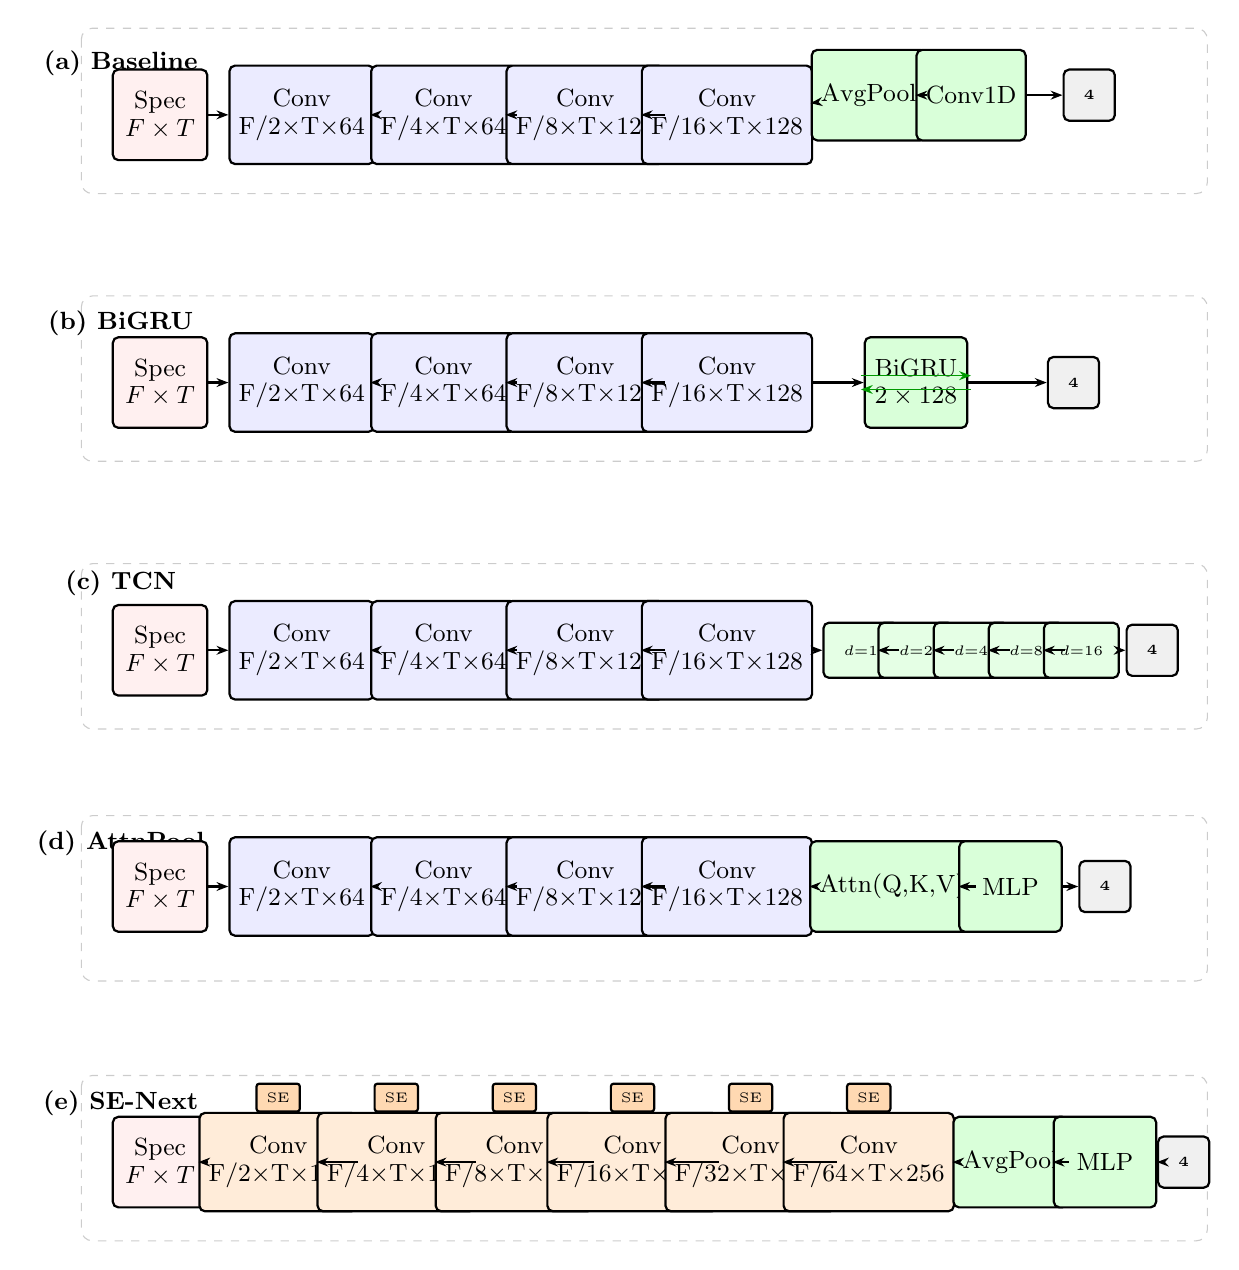
\begin{tikzpicture}[
  x=1cm, y=1cm,
  font=\small,
  encblock/.style={rectangle, draw, thick, fill=blue!8, rounded corners=2pt, minimum width=1.55cm, minimum height=1.25cm, align=center},
  modblock/.style={rectangle, draw, thick, fill=orange!15, rounded corners=2pt, minimum width=1.55cm, minimum height=1.25cm, align=center},
  headblock/.style={rectangle, draw, thick, fill=green!15, rounded corners=2pt, minimum width=1.3cm, minimum height=1.15cm, align=center},
  smallhead/.style={rectangle, draw, thick, fill=green!10, rounded corners=2pt, minimum width=0.95cm, minimum height=0.7cm, align=center, font=\tiny},
  inputblock/.style={rectangle, draw, thick, fill=red!6, rounded corners=2pt, minimum width=1.2cm, minimum height=1.15cm, align=center},
  outblock/.style={rectangle, draw, thick, fill=gray!12, rounded corners=2pt, minimum width=0.65cm, minimum height=0.65cm, align=center, font=\bfseries\tiny},
  seblock/.style={rectangle, draw, thick, fill=orange!30, rounded corners=1pt, minimum width=0.55cm, minimum height=0.35cm, align=center, font=\tiny},
  arrow/.style={-{Stealth[length=1.5mm]}, thick},
  label/.style={font=\bfseries\small},
  dashframe/.style={gray!40, dashed, rounded corners=4pt},
]

% ========== Row 1: Baseline ==========
\draw[dashframe] (-7.8,1.1) rectangle (6.5,-1.0);
\node[label] at (-7.3,0.65) {(a) Baseline};
\node[inputblock] (a-in) at (-6.8,0) {Spec\\[-1pt]$F\times T$};
\node[encblock] (a-b1) at (-5.0,0) {Conv\\[-1pt]\shapetext{F/2$\times$T$\times$64}};
\node[encblock] (a-b2) at (-3.2,0) {Conv\\[-1pt]\shapetext{F/4$\times$T$\times$64}};
\node[encblock] (a-b3) at (-1.4,0) {Conv\\[-1pt]\shapetext{F/8$\times$T$\times$128}};
\node[encblock] (a-b4) at (0.4,0) {Conv\\[-1pt]\shapetext{F/16$\times$T$\times$128}};
\node[headblock] (a-h1) at (2.2,0.25) {AvgPool};
\node[headblock] (a-h2) at (3.5,0.25) {Conv1D};
\node[outblock] (a-out) at (5.0,0.25) {4};
\draw[arrow] (a-in) -- (a-b1);
\draw[arrow] (a-b1) -- (a-b2);
\draw[arrow] (a-b2) -- (a-b3);
\draw[arrow] (a-b3) -- (a-b4);
\draw[arrow] (a-b4) -- (a-h1);
\draw[arrow] (a-h1) -- (a-h2);
\draw[arrow] (a-h2) -- (a-out);

% ========== Row 2: BiGRU ==========
\draw[dashframe] (-7.8,-2.3) rectangle (6.5,-4.4);
\node[label] at (-7.3,-2.65) {(b) BiGRU};
\node[inputblock] (b-in) at (-6.8,-3.4) {Spec\\[-1pt]$F\times T$};
\node[encblock] (b-b1) at (-5.0,-3.4) {Conv\\[-1pt]\shapetext{F/2$\times$T$\times$64}};
\node[encblock] (b-b2) at (-3.2,-3.4) {Conv\\[-1pt]\shapetext{F/4$\times$T$\times$64}};
\node[encblock] (b-b3) at (-1.4,-3.4) {Conv\\[-1pt]\shapetext{F/8$\times$T$\times$128}};
\node[encblock] (b-b4) at (0.4,-3.4) {Conv\\[-1pt]\shapetext{F/16$\times$T$\times$128}};
\node[headblock] (b-h) at (2.8,-3.4) {BiGRU\\[-1pt]\shapetext{$2\times128$}};
\node[outblock] (b-out) at (4.8,-3.4) {4};
\draw[arrow] (b-in) -- (b-b1);
\draw[arrow] (b-b1) -- (b-b2);
\draw[arrow] (b-b2) -- (b-b3);
\draw[arrow] (b-b3) -- (b-b4);
\draw[arrow] (b-b4) -- (b-h);
\draw[arrow] (b-h) -- (b-out);
% Bidirectional arrows on BiGRU
\draw[arrow, green!60!black, line width=0.5pt] ([yshift=2.5pt,xshift=-1pt]b-h.west) -- ([yshift=2.5pt,xshift=1pt]b-h.east);
\draw[arrow, green!60!black, line width=0.5pt] ([yshift=-2.5pt,xshift=1pt]b-h.east) -- ([yshift=-2.5pt,xshift=-1pt]b-h.west);

% ========== Row 3: TCN ==========
\draw[dashframe] (-7.8,-5.7) rectangle (6.5,-7.8);
\node[label] at (-7.3,-5.95) {(c) TCN};
\node[inputblock] (c-in) at (-6.8,-6.8) {Spec\\[-1pt]$F\times T$};
\node[encblock] (c-b1) at (-5.0,-6.8) {Conv\\[-1pt]\shapetext{F/2$\times$T$\times$64}};
\node[encblock] (c-b2) at (-3.2,-6.8) {Conv\\[-1pt]\shapetext{F/4$\times$T$\times$64}};
\node[encblock] (c-b3) at (-1.4,-6.8) {Conv\\[-1pt]\shapetext{F/8$\times$T$\times$128}};
\node[encblock] (c-b4) at (0.4,-6.8) {Conv\\[-1pt]\shapetext{F/16$\times$T$\times$128}};
\node[smallhead] (c-d1) at (2.1,-6.8) {$d$=1};
\node[smallhead] (c-d2) at (2.8,-6.8) {$d$=2};
\node[smallhead] (c-d3) at (3.5,-6.8) {$d$=4};
\node[smallhead] (c-d4) at (4.2,-6.8) {$d$=8};
\node[smallhead] (c-d5) at (4.9,-6.8) {$d$=16};
\node[outblock] (c-out) at (5.8,-6.8) {4};
\draw[arrow] (c-in) -- (c-b1);
\draw[arrow] (c-b1) -- (c-b2);
\draw[arrow] (c-b2) -- (c-b3);
\draw[arrow] (c-b3) -- (c-b4);
\draw[arrow] (c-b4) -- (c-d1);
\draw[arrow] (c-d1) -- (c-d2);
\draw[arrow] (c-d2) -- (c-d3);
\draw[arrow] (c-d3) -- (c-d4);
\draw[arrow] (c-d4) -- (c-d5);
\draw[arrow] (c-d5) -- (c-out);

% ========== Row 4: AttnPool ==========
\draw[dashframe] (-7.8,-8.9) rectangle (6.5,-11.0);
\node[label] at (-7.3,-9.25) {(d) AttnPool};
\node[inputblock] (d-in) at (-6.8,-9.8) {Spec\\[-1pt]$F\times T$};
\node[encblock] (d-b1) at (-5.0,-9.8) {Conv\\[-1pt]\shapetext{F/2$\times$T$\times$64}};
\node[encblock] (d-b2) at (-3.2,-9.8) {Conv\\[-1pt]\shapetext{F/4$\times$T$\times$64}};
\node[encblock] (d-b3) at (-1.4,-9.8) {Conv\\[-1pt]\shapetext{F/8$\times$T$\times$128}};
\node[encblock] (d-b4) at (0.4,-9.8) {Conv\\[-1pt]\shapetext{F/16$\times$T$\times$128}};
\node[headblock] (d-h1) at (2.5,-9.8) {Attn(Q,K,V)};
\node[headblock] (d-h2) at (4.0,-9.8) {MLP};
\node[outblock] (d-out) at (5.2,-9.8) {4};
\draw[arrow] (d-in) -- (d-b1);
\draw[arrow] (d-b1) -- (d-b2);
\draw[arrow] (d-b2) -- (d-b3);
\draw[arrow] (d-b3) -- (d-b4);
\draw[arrow] (d-b4) -- (d-h1);
\draw[arrow] (d-h1) -- (d-h2);
\draw[arrow] (d-h2) -- (d-out);

% ========== Row 5: SE-Next ==========
\draw[dashframe] (-7.8,-12.2) rectangle (6.5,-14.3);
\node[label] at (-7.3,-12.55) {(e) SE-Next};
\node[inputblock] (e-in) at (-6.8,-13.3) {Spec\\[-1pt]$F\times T$};
\node[modblock] (e-b1) at (-5.3,-13.3) {Conv\\[-1pt]\shapetext{F/2$\times$T$\times$128}};
\node[modblock] (e-b2) at (-3.8,-13.3) {Conv\\[-1pt]\shapetext{F/4$\times$T$\times$128}};
\node[modblock] (e-b3) at (-2.3,-13.3) {Conv\\[-1pt]\shapetext{F/8$\times$T$\times$128}};
\node[modblock] (e-b4) at (-0.8,-13.3) {Conv\\[-1pt]\shapetext{F/16$\times$T$\times$256}};
\node[modblock] (e-b5) at (0.7,-13.3) {Conv\\[-1pt]\shapetext{F/32$\times$T$\times$256}};
\node[modblock] (e-b6) at (2.2,-13.3) {Conv\\[-1pt]\shapetext{F/64$\times$T$\times$256}};
\node[seblock] at ([yshift=0.18cm]e-b1.north) {SE};
\node[seblock] at ([yshift=0.18cm]e-b2.north) {SE};
\node[seblock] at ([yshift=0.18cm]e-b3.north) {SE};
\node[seblock] at ([yshift=0.18cm]e-b4.north) {SE};
\node[seblock] at ([yshift=0.18cm]e-b5.north) {SE};
\node[seblock] at ([yshift=0.18cm]e-b6.north) {SE};
\node[headblock] (e-h1) at (4.0,-13.3) {AvgPool};
\node[headblock] (e-h2) at (5.2,-13.3) {MLP};
\node[outblock] (e-out) at (6.2,-13.3) {4};
\draw[arrow] (e-in) -- (e-b1);
\draw[arrow] (e-b1) -- (e-b2);
\draw[arrow] (e-b2) -- (e-b3);
\draw[arrow] (e-b3) -- (e-b4);
\draw[arrow] (e-b4) -- (e-b5);
\draw[arrow] (e-b5) -- (e-b6);
\draw[arrow] (e-b6) -- (e-h1);
\draw[arrow] (e-h1) -- (e-h2);
\draw[arrow] (e-h2) -- (e-out);

\end{tikzpicture}
\caption{Architectural variants (a)--(e).  Each row shows the full data-flow from input spectrogram to four rotor-speed outputs.  Block labels give the tensor shape (frequency $\times$ time $\times$ channels) after each encoder stage.  Small orange \texttt{SE} blocks are squeeze--excitation modules.}
\label{fig:arch-variants-1}
\end{figure}

\begin{figure}[p]
\centering
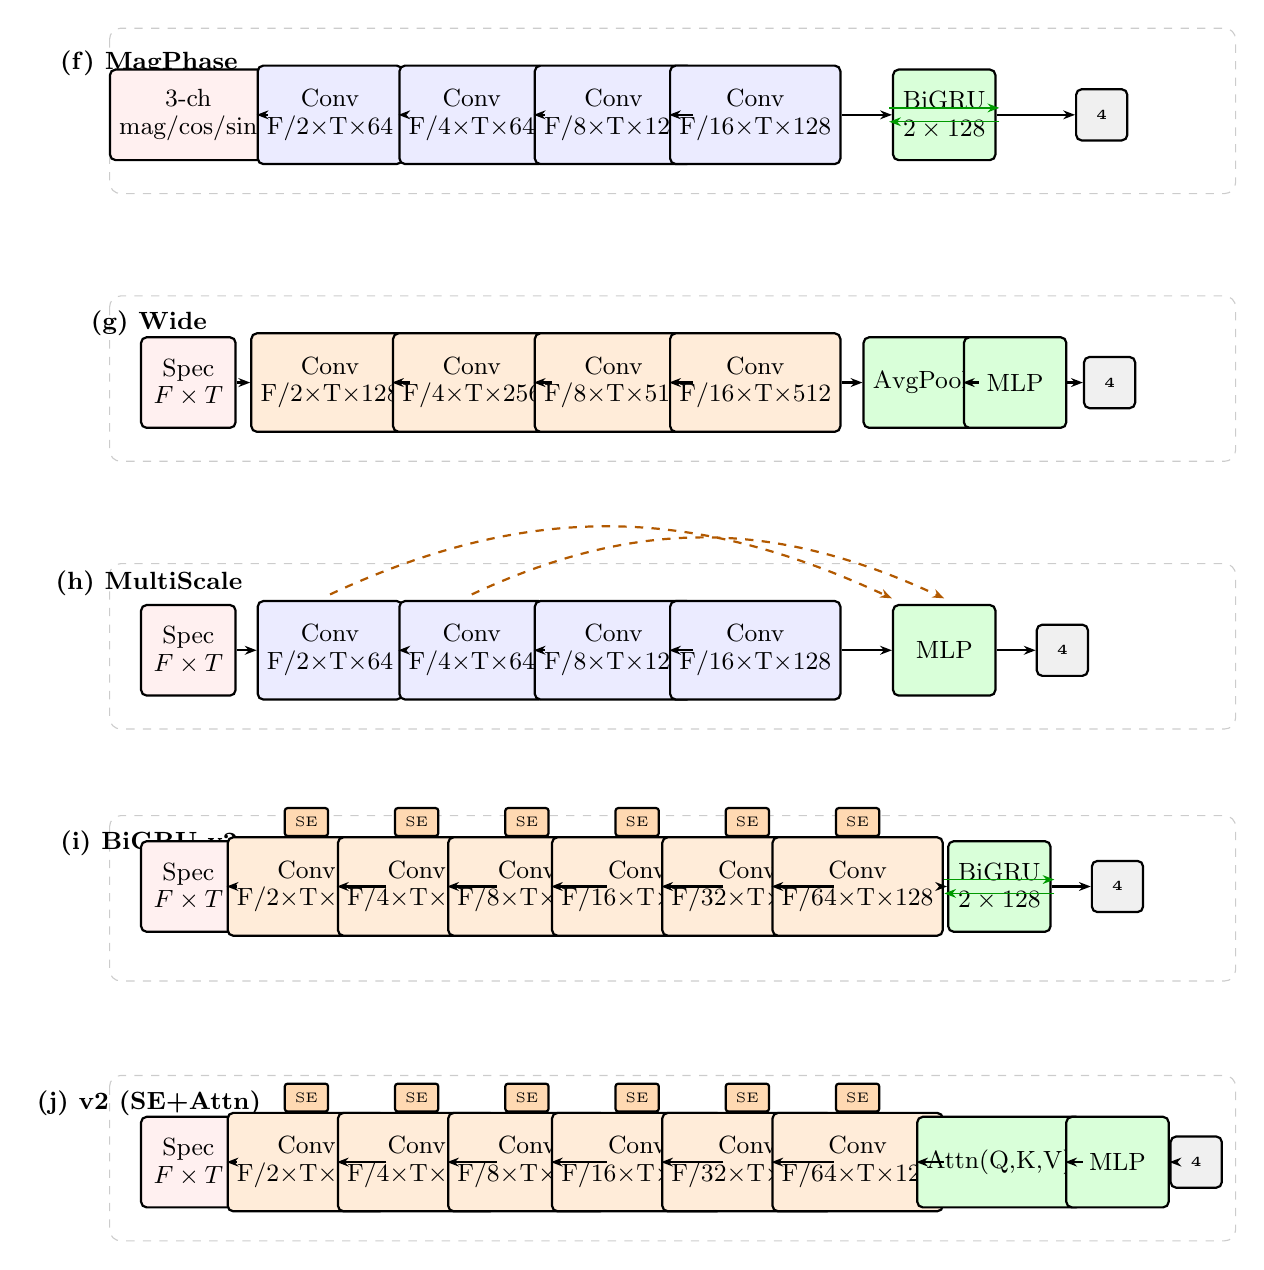
\begin{tikzpicture}[
  x=1cm, y=1cm,
  font=\small,
  encblock/.style={rectangle, draw, thick, fill=blue!8, rounded corners=2pt, minimum width=1.55cm, minimum height=1.25cm, align=center},
  modblock/.style={rectangle, draw, thick, fill=orange!15, rounded corners=2pt, minimum width=1.55cm, minimum height=1.25cm, align=center},
  headblock/.style={rectangle, draw, thick, fill=green!15, rounded corners=2pt, minimum width=1.3cm, minimum height=1.15cm, align=center},
  smallhead/.style={rectangle, draw, thick, fill=green!10, rounded corners=2pt, minimum width=0.95cm, minimum height=0.7cm, align=center, font=\tiny},
  inputblock/.style={rectangle, draw, thick, fill=red!6, rounded corners=2pt, minimum width=1.2cm, minimum height=1.15cm, align=center},
  outblock/.style={rectangle, draw, thick, fill=gray!12, rounded corners=2pt, minimum width=0.65cm, minimum height=0.65cm, align=center, font=\bfseries\tiny},
  seblock/.style={rectangle, draw, thick, fill=orange!30, rounded corners=1pt, minimum width=0.55cm, minimum height=0.35cm, align=center, font=\tiny},
  arrow/.style={-{Stealth[length=1.5mm]}, thick},
  label/.style={font=\bfseries\small},
  dashframe/.style={gray!40, dashed, rounded corners=4pt},
]

% ========== Row 6: MagPhase ==========
\draw[dashframe] (-7.8,1.1) rectangle (6.5,-1.0);
\node[label] at (-7.3,0.65) {(f) MagPhase};
\node[inputblock] (f-in) at (-6.8,0) {3-ch\\[-1pt]mag/cos/sin};
\node[encblock] (f-b1) at (-5.0,0) {Conv\\[-1pt]\shapetext{F/2$\times$T$\times$64}};
\node[encblock] (f-b2) at (-3.2,0) {Conv\\[-1pt]\shapetext{F/4$\times$T$\times$64}};
\node[encblock] (f-b3) at (-1.4,0) {Conv\\[-1pt]\shapetext{F/8$\times$T$\times$128}};
\node[encblock] (f-b4) at (0.4,0) {Conv\\[-1pt]\shapetext{F/16$\times$T$\times$128}};
\node[headblock] (f-h) at (2.8,0) {BiGRU\\[-1pt]\shapetext{$2\times128$}};
\node[outblock] (f-out) at (4.8,0) {4};
\draw[arrow] (f-in) -- (f-b1);
\draw[arrow] (f-b1) -- (f-b2);
\draw[arrow] (f-b2) -- (f-b3);
\draw[arrow] (f-b3) -- (f-b4);
\draw[arrow] (f-b4) -- (f-h);
\draw[arrow] (f-h) -- (f-out);
\draw[arrow, green!60!black, line width=0.5pt] ([yshift=2.5pt,xshift=-1pt]f-h.west) -- ([yshift=2.5pt,xshift=1pt]f-h.east);
\draw[arrow, green!60!black, line width=0.5pt] ([yshift=-2.5pt,xshift=1pt]f-h.east) -- ([yshift=-2.5pt,xshift=-1pt]f-h.west);

% ========== Row 7: Wide ==========
\draw[dashframe] (-7.8,-2.3) rectangle (6.5,-4.4);
\node[label] at (-7.3,-2.65) {(g) Wide};
\node[inputblock] (g-in) at (-6.8,-3.4) {Spec\\[-1pt]$F\times T$};
\node[modblock] (g-b1) at (-5.0,-3.4) {Conv\\[-1pt]\shapetext{F/2$\times$T$\times$128}};
\node[modblock] (g-b2) at (-3.2,-3.4) {Conv\\[-1pt]\shapetext{F/4$\times$T$\times$256}};
\node[modblock] (g-b3) at (-1.4,-3.4) {Conv\\[-1pt]\shapetext{F/8$\times$T$\times$512}};
\node[modblock] (g-b4) at (0.4,-3.4) {Conv\\[-1pt]\shapetext{F/16$\times$T$\times$512}};
\node[headblock] (g-h1) at (2.5,-3.4) {AvgPool};
\node[headblock] (g-h2) at (3.7,-3.4) {MLP};
\node[outblock] (g-out) at (4.9,-3.4) {4};
\draw[arrow] (g-in) -- (g-b1);
\draw[arrow] (g-b1) -- (g-b2);
\draw[arrow] (g-b2) -- (g-b3);
\draw[arrow] (g-b3) -- (g-b4);
\draw[arrow] (g-b4) -- (g-h1);
\draw[arrow] (g-h1) -- (g-h2);
\draw[arrow] (g-h2) -- (g-out);

% ========== Row 8: MultiScale ==========
\draw[dashframe] (-7.8,-5.7) rectangle (6.5,-7.8);
\node[label] at (-7.3,-5.95) {(h) MultiScale};
\node[inputblock] (h-in) at (-6.8,-6.8) {Spec\\[-1pt]$F\times T$};
\node[encblock] (h-b1) at (-5.0,-6.8) {Conv\\[-1pt]\shapetext{F/2$\times$T$\times$64}};
\node[encblock] (h-b2) at (-3.2,-6.8) {Conv\\[-1pt]\shapetext{F/4$\times$T$\times$64}};
\node[encblock] (h-b3) at (-1.4,-6.8) {Conv\\[-1pt]\shapetext{F/8$\times$T$\times$128}};
\node[encblock] (h-b4) at (0.4,-6.8) {Conv\\[-1pt]\shapetext{F/16$\times$T$\times$128}};
\node[headblock] (h-h) at (2.8,-6.8) {MLP};
\node[outblock] (h-out) at (4.3,-6.8) {4};
\draw[arrow] (h-in) -- (h-b1);
\draw[arrow] (h-b1) -- (h-b2);
\draw[arrow] (h-b2) -- (h-b3);
\draw[arrow] (h-b3) -- (h-b4);
\draw[arrow] (h-b4) -- (h-h);
\draw[arrow] (h-h) -- (h-out);
% FPN skip connections
\draw[arrow, orange!70!black, dashed, thick] ([yshift=2pt]h-b1.north) to[out=25,in=155] ([yshift=2pt]h-h.north west);
\draw[arrow, orange!70!black, dashed, thick] ([yshift=2pt]h-b2.north) to[out=25,in=155] ([yshift=2pt]h-h.north);

% ========== Row 9: BiGRU-v2 ==========
\draw[dashframe] (-7.8,-8.9) rectangle (6.5,-11.0);
\node[label] at (-7.3,-9.25) {(i) BiGRU-v2};
\node[inputblock] (i-in) at (-6.8,-9.8) {Spec\\[-1pt]$F\times T$};
\node[modblock] (i-b1) at (-5.3,-9.8) {Conv\\[-1pt]\shapetext{F/2$\times$T$\times$128}};
\node[modblock] (i-b2) at (-3.9,-9.8) {Conv\\[-1pt]\shapetext{F/4$\times$T$\times$128}};
\node[modblock] (i-b3) at (-2.5,-9.8) {Conv\\[-1pt]\shapetext{F/8$\times$T$\times$128}};
\node[modblock] (i-b4) at (-1.1,-9.8) {Conv\\[-1pt]\shapetext{F/16$\times$T$\times$128}};
\node[modblock] (i-b5) at (0.3,-9.8) {Conv\\[-1pt]\shapetext{F/32$\times$T$\times$128}};
\node[modblock] (i-b6) at (1.7,-9.8) {Conv\\[-1pt]\shapetext{F/64$\times$T$\times$128}};
\node[seblock] at ([yshift=0.18cm]i-b1.north) {SE};
\node[seblock] at ([yshift=0.18cm]i-b2.north) {SE};
\node[seblock] at ([yshift=0.18cm]i-b3.north) {SE};
\node[seblock] at ([yshift=0.18cm]i-b4.north) {SE};
\node[seblock] at ([yshift=0.18cm]i-b5.north) {SE};
\node[seblock] at ([yshift=0.18cm]i-b6.north) {SE};
\node[headblock] (i-h) at (3.5,-9.8) {BiGRU\\[-1pt]\shapetext{$2\times128$}};
\node[outblock] (i-out) at (5.0,-9.8) {4};
\draw[arrow] (i-in) -- (i-b1);
\draw[arrow] (i-b1) -- (i-b2);
\draw[arrow] (i-b2) -- (i-b3);
\draw[arrow] (i-b3) -- (i-b4);
\draw[arrow] (i-b4) -- (i-b5);
\draw[arrow] (i-b5) -- (i-b6);
\draw[arrow] (i-b6) -- (i-h);
\draw[arrow] (i-h) -- (i-out);
\draw[arrow, green!60!black, line width=0.5pt] ([yshift=2.5pt,xshift=-1pt]i-h.west) -- ([yshift=2.5pt,xshift=1pt]i-h.east);
\draw[arrow, green!60!black, line width=0.5pt] ([yshift=-2.5pt,xshift=1pt]i-h.east) -- ([yshift=-2.5pt,xshift=-1pt]i-h.west);

% ========== Row 10: v2 (SE+Attn) ==========
\draw[dashframe] (-7.8,-12.2) rectangle (6.5,-14.3);
\node[label] at (-7.3,-12.55) {(j) v2 (SE+Attn)};
\node[inputblock] (j-in) at (-6.8,-13.3) {Spec\\[-1pt]$F\times T$};
\node[modblock] (j-b1) at (-5.3,-13.3) {Conv\\[-1pt]\shapetext{F/2$\times$T$\times$128}};
\node[modblock] (j-b2) at (-3.9,-13.3) {Conv\\[-1pt]\shapetext{F/4$\times$T$\times$128}};
\node[modblock] (j-b3) at (-2.5,-13.3) {Conv\\[-1pt]\shapetext{F/8$\times$T$\times$128}};
\node[modblock] (j-b4) at (-1.1,-13.3) {Conv\\[-1pt]\shapetext{F/16$\times$T$\times$128}};
\node[modblock] (j-b5) at (0.3,-13.3) {Conv\\[-1pt]\shapetext{F/32$\times$T$\times$128}};
\node[modblock] (j-b6) at (1.7,-13.3) {Conv\\[-1pt]\shapetext{F/64$\times$T$\times$128}};
\node[seblock] at ([yshift=0.18cm]j-b1.north) {SE};
\node[seblock] at ([yshift=0.18cm]j-b2.north) {SE};
\node[seblock] at ([yshift=0.18cm]j-b3.north) {SE};
\node[seblock] at ([yshift=0.18cm]j-b4.north) {SE};
\node[seblock] at ([yshift=0.18cm]j-b5.north) {SE};
\node[seblock] at ([yshift=0.18cm]j-b6.north) {SE};
\node[headblock] (j-h1) at (3.5,-13.3) {Attn(Q,K,V)};
\node[headblock] (j-h2) at (5.0,-13.3) {MLP};
\node[outblock] (j-out) at (6.0,-13.3) {4};
\draw[arrow] (j-in) -- (j-b1);
\draw[arrow] (j-b1) -- (j-b2);
\draw[arrow] (j-b2) -- (j-b3);
\draw[arrow] (j-b3) -- (j-b4);
\draw[arrow] (j-b4) -- (j-b5);
\draw[arrow] (j-b5) -- (j-b6);
\draw[arrow] (j-b6) -- (j-h1);
\draw[arrow] (j-h1) -- (j-h2);
\draw[arrow] (j-h2) -- (j-out);

\end{tikzpicture}
\caption{Architectural variants (f)--(j).  Colour key as in Figure~\ref{fig:arch-variants-1}.  Dashed orange arrows in (h) are FPN skip connections.}
\label{fig:arch-variants-2}
\end{figure}

% ============================================================================
\section{Validation-set results}
% ============================================================================

\begin{table}[ht]
  \centering
  \caption{Leaderboard on the 600-clip DREGON-LM validation set.}
  \label{tab:leaderboard}
  \small
  \begin{tabular}{clcccc}
    \toprule
    Rank & Model & MSE$\downarrow$ & RMSE & MAE$\downarrow$ & $\rsq\uparrow$ \\
    \midrule
    1 & v2 (SE+Attn) & 2.61 & 1.61 & 0.76 & \textbf{0.951} \\
    2 & BiGRU-v2 & 2.67 & 1.64 & 0.78 & 0.948 \\
    3 & BiGRU & 2.74 & 1.66 & 0.80 & 0.945 \\
    4 & TCN & 3.09 & 1.76 & 0.83 & 0.936 \\
    5 & MagPhase & 3.16 & 1.78 & 0.96 & 0.917 \\
    6 & AttnPool & 4.87 & 2.21 & 1.25 & 0.860 \\
    7 & Wide & 5.04 & 2.24 & 1.32 & 0.847 \\
    8 & MultiScale & 5.15 & 2.27 & 1.31 & 0.840 \\
    9 & Baseline & 5.21 & 2.28 & 1.36 & 0.837 \\
    10 & SE-Next & 7.30 & 2.70 & 1.86 & 0.688 \\
    \bottomrule
  \end{tabular}
\end{table}

\begin{figure}[ht]
  \centering
  
\includegraphics[width=\textwidth]{fig_leaderboard_validation}
  \caption{(a) Validation MSE and (b) coefficient of determination for all ten variants.}
  \label{fig:leaderboard}
\end{figure}

\begin{figure}[ht]
  \centering
  
\includegraphics[width=0.65\textwidth]{fig_pareto_params_r2}
  \caption{Pareto frontier: parameter count vs. validation $\rsq$.}
  \label{fig:pareto}
\end{figure}

% ============================================================================
\section{Full-sequence evaluation}
% ============================================================================

We evaluate on the DREGON \emph{free-flight speech-high room1} recording ($\sim$47~s). The in-flight metric excludes takeoff/landing ($\rps < 50$~\revps{}), where all models fail due to distribution shift.

\begin{table}[ht]
  \centering
  \caption{Full-sequence metrics.}
  \label{tab:fullseq}
  \small
  \begin{tabular}{lccc}
    \toprule
    Model & Global MSE & In-flight MSE$\downarrow$ & Global $\rsq$ \\
    \midrule
    BiGRU-v2 & 73.60 & \textbf{9.90} & \textbf{0.839} \\
    v2 (SE+Attn) & 137.48 & 11.80 & 0.700 \\
    BiGRU & 104.10 & 15.19 & 0.772 \\
    Wide & 106.85 & 18.87 & 0.766 \\
    AttnPool & 110.88 & 19.99 & 0.758 \\
    Baseline & 104.14 & 24.45 & 0.772 \\
    SE-Next & 113.67 & 23.44 & 0.752 \\
    MagPhase & 91.71 & 25.73 & 0.800 \\
    TCN & 105.82 & 28.14 & 0.769 \\
    MultiScale & 1940.89 & 111.71 & $-0.862$ \\
    \bottomrule
  \end{tabular}
\end{table}

\begin{figure}[ht]
  \centering
  
\includegraphics[width=\textwidth]{fig_fullsequence_comparison}
  \caption{Multi-variant overlay on the full-sequence recording. Top: mean predicted rotor speed. Bottom: per-frame MSE (1-s smoothed).}
  \label{fig:fullseq}
\end{figure}

\begin{figure}[ht]
  \centering
  
\includegraphics[width=0.8\textwidth]{fig_fullsequence_inflight_mse_bar}
  \caption{In-flight MSE on the real recording. BiGRU-v2 halves the baseline error.}
  \label{fig:fullseq-bar}
\end{figure}

\begin{figure}[ht]
  \centering
  \includegraphics[width=\textwidth]{fig_fullsequence_simple_conv_bigru_v2}
  \caption{BiGRU-v2: 3-panel full-sequence plot (spectrogram, traces, per-frame MSE).}
  \label{fig:fullseq-bigru-v2}
\end{figure}

% ============================================================================
\section{Individual-motor and allMotors tests}
% ============================================================================

All models were trained on four-rotor mixtures with varying speeds. On clean single-rotor recordings they fail catastrophically (MSE in the thousands), confirming a strong structural prior.

\begin{figure}[ht]
  \centering
  
\includegraphics[width=\textwidth]{fig_individual_motor_mse_bar}
  \caption{Best-channel MSE on individual-motor recordings. All variants fail by two to three orders of magnitude.}
  \label{fig:individual}
\end{figure}

On \texttt{allMotors\_70} (four synchronized rotors at 70~\revps{}) the models recover because the input matches their structural expectation:

\begin{table}[ht]
  \centering
  \caption{allMotors\_70 results.}
  \label{tab:allmotors}
  \small
  \begin{tabular}{lcc}
    \toprule
    Model & Best MSE$\downarrow$ & Avg MSE$\downarrow$ \\
    \midrule
    MultiScale & 16.10 & 28.93 \\
    Baseline & 22.26 & 91.07 \\
    Wide & 22.24 & 85.26 \\
    BiGRU-v2 & 22.30 & 89.29 \\
    SE-Next & 24.12 & 94.10 \\
    TCN & 28.96 & 65.85 \\
    AttnPool & 30.06 & 113.03 \\
    v2 (SE+Attn) & 316.55 & 347.13 \\
    BiGRU & 392.28 & 416.77 \\
    MagPhase & 640.30 & 676.49 \\
    \bottomrule
  \end{tabular}
\end{table}

\begin{figure}[ht]
  \centering
  
\includegraphics[width=\textwidth]{fig_single_rotor_allmotors_comparison}
  \caption{Predictions on allMotors\_70 for five representative variants. Dotted = four channels; solid = mean; bold = best channel.}
  \label{fig:allmotors-traces}
\end{figure}

\begin{figure}[ht]
  \centering
  
\includegraphics[width=0.85\textwidth]{fig_allmotors_mse_bar}
  \caption{allMotors\_70 MSE: best channel vs. mean over four channels.}
  \label{fig:allmotors-bar}
\end{figure}

% ============================================================================
\section{Discussion and recommendation}
% ============================================================================

\paragraph{What works.}
(1)~The BiGRU temporal head is the dominant improvement (+0.108 $\rsq$ over baseline). Every top-5 model has it. (2)~A deeper encoder with SE blocks improves generalisation: BiGRU-v2 matches v2 on validation but wins decisively on the real recording (in-flight MSE 9.9 vs 11.8). (3)~TCN is the best non-recurrent architecture ($\rsq = 0.936$).

\paragraph{What does not.}
SE-Next without temporal modelling is worse than baseline ($\rsq = 0.688$). Width scaling (3.94M params) barely helps. Phase input adds complexity without gain. Multi-scale fusion is unstable and breaks temporal resolution.

\paragraph{Practical choice.}
For downstream speech-enhancement pipelines that depend on accurate \rps{} conditioning, \textbf{SimpleConv-BiGRU-v2} offers the best trade-off: strongest real-recording performance (in-flight MSE 9.9), competitive validation accuracy ($\rsq = 0.948$), and moderate size (1.44M params). If parameter count is critical, \textbf{SimpleConv-BiGRU} (0.67M params, $\rsq = 0.945$) provides 99.4\% of v2's validation performance at 44\% of the parameters, with real-recording in-flight MSE of 15.2.

\end{document}
